%!TEX TS-program = xelatex
\documentclass{beamer}

\usepackage{HSE-theme/beamerthemeHSE} % Подгружаем тему

%%% Работа с русским языком и шрифтами
\usepackage[english,russian]{babel}   % загружает пакет многоязыковой вёрстки
\usepackage{fontspec}      % подготавливает загрузку шрифтов Open Type, True Type и др.

\defaultfontfeatures{Ligatures={TeX},Renderer=Basic}  % свойства шрифтов по умолчанию
% \setmainfont[Ligatures={TeX,Historic}]{KanjiStrokeOrders.ttf} %  установите шрифты Myriad Pro или (при невозможности) замените здесь на другой шрифт, который есть в системе — например, Arial
\setmainfont[ExternalLocation={./},Ligatures={TeX,Historic}]{MyriadPro-Regular.otf} %  установите шрифты Myriad Pro или (при невозможности) замените здесь на другой шрифт, который есть в системе — например, Arial
\setsansfont[ExternalLocation={./}]{MyriadPro-Regular.otf} %  установите шрифты Myriad Pro или (при невозможности) замените здесь на другой шрифт, который есть в системе — например, Arial
\setmonofont[ExternalLocation={./}]{MyriadPro-Regular.otf}
%\setmonofont{Courier New}

\uselanguage{russian}
\languagepath{russian}
\deftranslation[to=russian]{Theorem}{Теорема}
\deftranslation[to=russian]{Definition}{Определение}
\deftranslation[to=russian]{Definitions}{Определения}
\deftranslation[to=russian]{Corollary}{Следствие}
\deftranslation[to=russian]{Fact}{Факт}
\deftranslation[to=russian]{Example}{Пример}
\deftranslation[to=russian]{Examples}{Примеры}

\usepackage{multicol} 		% Несколько колонок
\graphicspath{{images/}}  	% Папка с картинками

\usepackage{color}
\usepackage{listings}

% use this to excape underscores
\newcommand{\Code}[1]{\detokenize{#1}}

% use this to highlight in green for emphasis
\newcommand{\Green}[1]{\begin{exampleblock}#1\end{exampleblock}}

%%% Информация об авторе и выступлении
\title[Курсовая работа]{\scriptsize{%
Факультет компьютерных наук \\%
Департамент программной инженерии \\%
Курсовая работа \\%
}}

\subtitle{Программа скелетная анимация}

\author[Абрамов Артем 151 БПИ]{\scriptsize{%
Выполнил студент группы 151БПИ \\%
Абрамов Артем Михайлович \\%
Научный руководитель: \\%
доцент департамента программной \\%
инженерии, к.т.н \\%
Ахметсафина Римма Закиевна}}

%\institute[Высшая школа экономики]{Национальный исследовательский университет \\ «Высшая школа экономики» (Москва)}
\date{2016}

\begin{document}	% Начало презентации

\frame[plain]{\titlepage}	% Титульный слайд

%\section{Просто слайд с текстом}
%\subsection{Просто слайд с текстом}



%=============================================================
\begin{frame}
\frametitle{Предметная область}
\begin{multicols}{2}
\begin{small}
    3-x мерная компьютерная анимация - вид мультипликации, создаваемый при помощи компьютера. 
    \medskip
    
    В отличии от 2-х мерной анимаци, художник не рисует каждый кадр, а работает с моделью для которой последовательно задает различные позы.

    \medskip 
    Отображение анимации - одна из наиболее актуальных задач  в производственной, научной и деловой сферах, а также в области развлечений.
\end{small}

\columnbreak
    
\begin{figure}[h!]
    \centering
    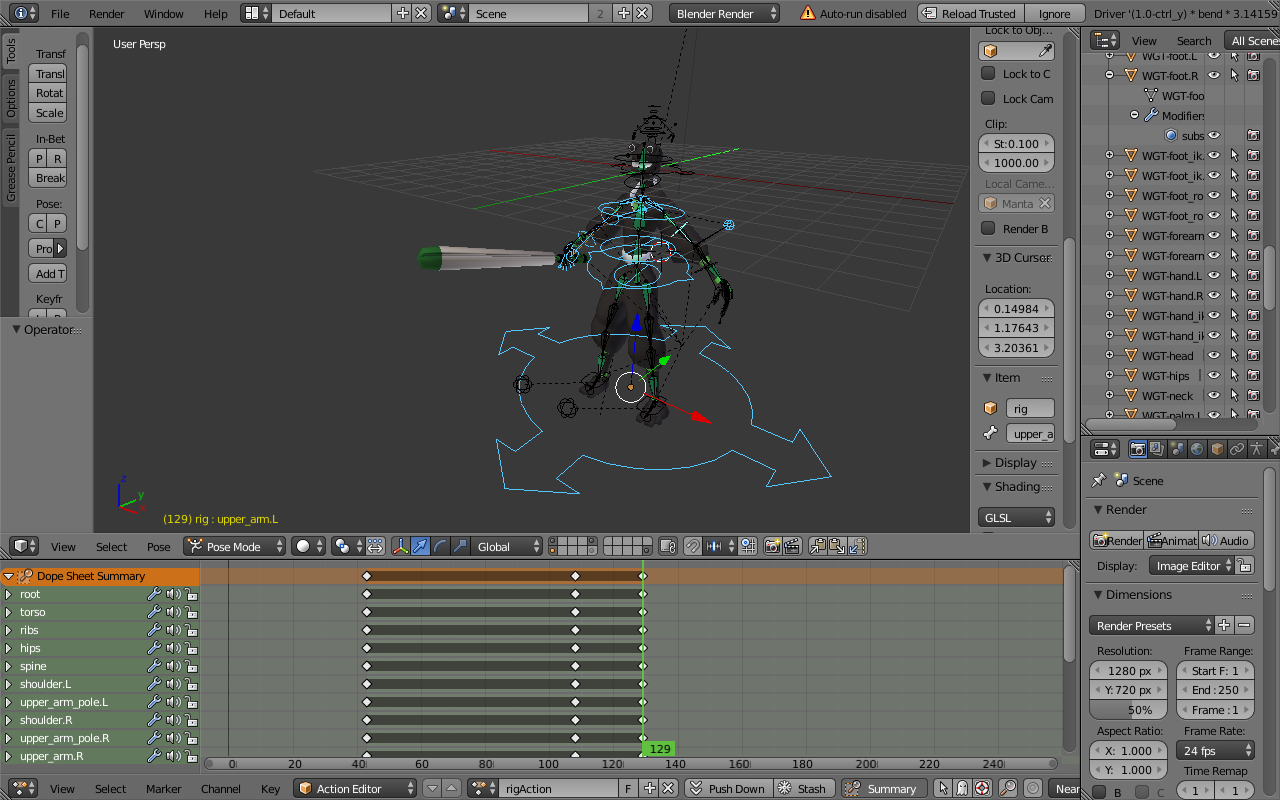
\includegraphics[width=1.15\columnwidth]{blender_at_work.png}
    \caption{Создание анимации в программе Blender}
    %\label{fig:awesome_image}
\end{figure}

\end{multicols}
\end{frame}


%=============================================================
\begin{frame}
\frametitle{Основные определения}
    
\end{frame}


%=============================================================
\begin{frame}
\frametitle{Обоснование актуальности работы}
    \begin{center}            
    \begin{large}
    ???
    \end{large}
    \end{center}
\end{frame}



%=============================================================
\begin{frame}
\frametitle{Цели и задачи работы}
    Цель работы - реализовать систему скелетной анимации.
    
    \bigskip
    
    Задачи работы
    
    \smallskip
	\begin{enumerate}
	\item Создание исходных данных (файлов) для скелетной анимации.
	\item Загрузка анимации из файла (содержание описанно в ТЗ).
	\item Рассчет кадров анимации.
	\item Воспроизведение анимации на экране средствами OpenGL.
	\end{enumerate}
    
\end{frame}



%=============================================================
\begin{frame}
\frametitle{Аналоги программы}
    \scriptsize{Пакеты 3-х мерного моделлирования. Maya, 3ds MAX, Blender, Cinema4D.}
\begin{figure}[h!]
    \centering
    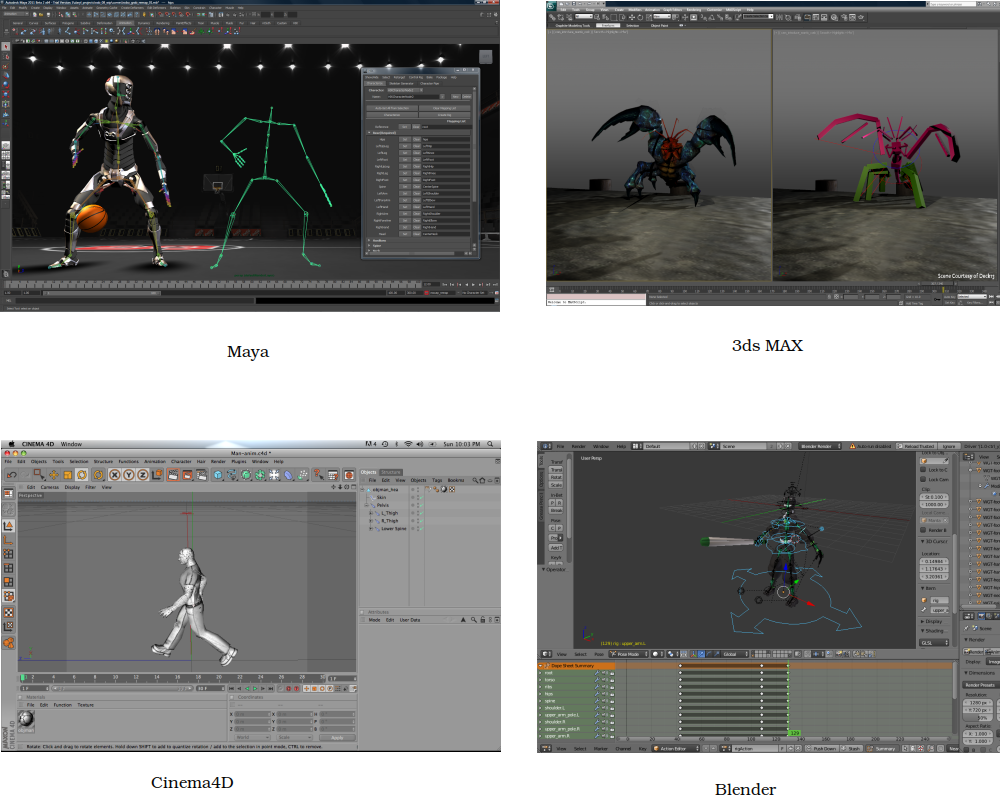
\includegraphics[width=0.8\textwidth]{all_tools.png}
    %\label{fig:awesome_image}
\end{figure}

\end{frame}



%=============================================================
\begin{frame}
\frametitle{Различные подходы}
\begin{small}
    Для 3-х мерной анимации не существует оптимального подхода. Все системы балансируют между методами с большим количеством вычислений и методами, требующими большого объема памяти.
    
    \medskip
    \alert{Неявные системы} используются, когда действия персонажа связанны с другими предметами, и нельзя предугадать все возможные варианты анимации. Например для того, чтобы ставить ступню параллельно поверхности при движении по неровной земле.
    
    \smallskip
    Предпочтение \alert{явным системам} отдается, когда необходимо анимировать большие группы людей или животных.
    
\begin{figure}[h!]
    \centering
    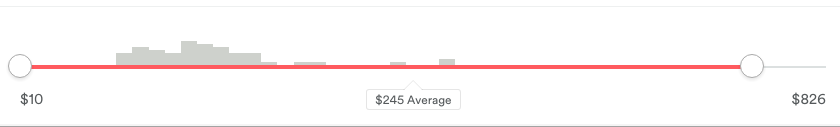
\includegraphics[width=1\textwidth]{raw_graph_cpu_vs_ram.png}
    %\caption{Шкала подходов к анимации, и отображающая позицию метода скелетной анимации}
    %\label{fig:awesome_image}
\end{figure}

\end{small}
\end{frame}



%=============================================================
\begin{frame}
\frametitle{Явные системы анимации}
\begin{scriptsize}
    Явная система - хранение отдельной модели для каждого кадра. \\
    После записи данных в файл, существует много методов для воспроизведения анимации.
    Такие методы требуют лишь элементарной математики. \\
    Однако типичная запись одного трэка анимации для одного персонажа занимает около 10MB (в формате MD3).
   
\begin{figure}[h!]
    \centering
    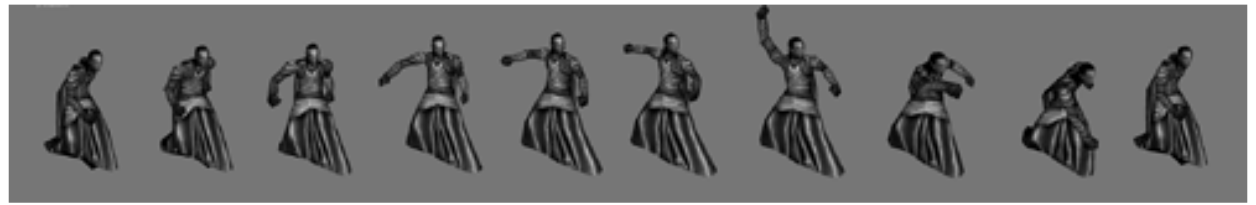
\includegraphics[width=1\textwidth]{explicit_animation.png}
    \caption{Каждому кадру соответствует своя модель}
\end{figure}

\end{scriptsize}
\end{frame}

  
%=============================================================
\begin{frame}
\frametitle{Неявные системы анимации}
\begin{scriptsize}
    Неявная система - хранение не моделей, а более высокоуровневого описания движения. \\
    В частности неявные \alert{системы скелетной анимации} содержат описание (через матрицу поворота) для каждой кости, как например локоть, плечо, шея. В реальном времени эти описания применяются к неанимированной модели для рассчета следующего кадра анимации. Эти рассчеты обычно требуют сложной математики с матрицами и тригонометрией. А следовательно и много CPU времени.
    
    \medskip
    Для реализации требуются 3 вещи: скелет, модель и трэк анимации. \\  
    Скелет определяет иерархию частей тела персонажа, в трэке содержатся матрицы для поворота скелета в ключевые моменты времени.
    
\begin{figure}[h!]
    \centering
    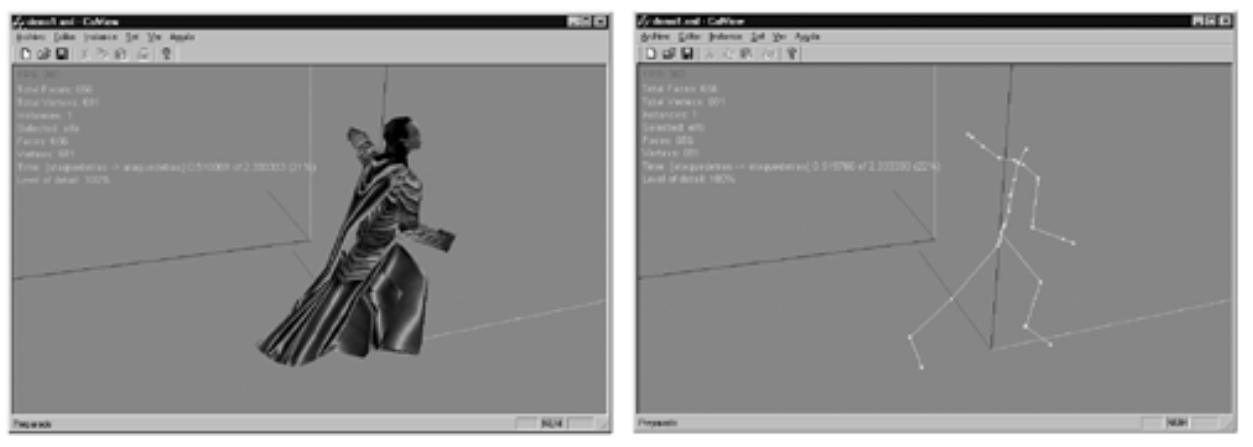
\includegraphics[width=0.8\textwidth]{implicit_animation.png}
    \caption{\scriptsize{Слева: анимированный персонаж; справа: скелет для данного кадра}}
    %\label{fig:awesome_image}
\end{figure}

\end{scriptsize}
\end{frame}



%=============================================================
\begin{frame}
\frametitle{Применение описания из трэка к скелету}
\begin{scriptsize}
    Матрицы поворота для всех костей записываются в трэке относительно матрицы поворота родителя.
Поэтому для деформации скелета необходимо применять матрицы последовательно.
Мы начинаем с корневой кости и применяем к ней описанную в трэке анимации матрицу поворота.
Затем, мы двигаемся вглубь скелета применяя матрицу родителя и деформацию описанную в трэке (то есть считаем глобальную матрицу поворота для данной кости).
    
\begin{figure}[h!]
    \centering
    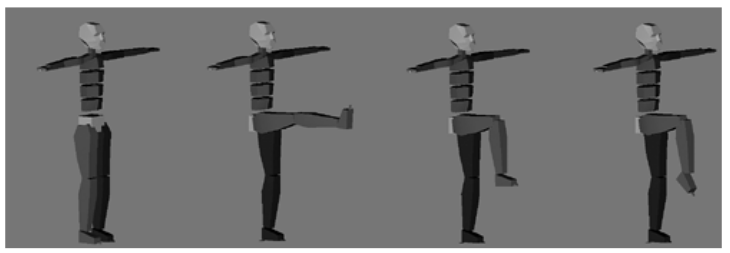
\includegraphics[width=1\textwidth]{forward_kinematics.png}
    \caption{\scriptsize{Применение преобразований, начиная от копчика (корневой кости) и заканчивая ступней.}}
    %\label{fig:awesome_image}
\end{figure}

\end{scriptsize}
\end{frame}


%=============================================================
\begin{frame}[fragile]
\frametitle{Применение деформации скелета к модели}

После того, как рассчитанны матрицы поворотов для скелета, их необходимо применить на вершины модели. Для этого используется рекурсивный алгоритм очень похожий на предыдущий.

\begin{scriptsize}
\begin{lstlisting}
deform (bone root, mesh original, mesh deformed)
  for each child_bone of root
    for each vertex in the original mesh
      if bone_weight > 0
          apply bone global transform to vertex
          scale the resulting point by the bone weight
          store the result in processeddata
      end if
    end for
    if child_bone has children
      deform (children of this node, mesh original, deformed)
    end if
  end for
\end{lstlisting}
\end{scriptsize}


\end{frame}


%=============================================================
\begin{frame}
\frametitle{Технологии и инструменты реализации}
\begin{itemize}
   \item Язык программирования C\#
   \item Библиотека \Code{Assimp v3.1 (http://assimp.org/)} для чтения файлов в формате collada (.dae).   
   \item Библиотека \Code{OpenTK v1.1.4 (http://www.opentk.com/)} для вызова функций OpenGL из C\# и предоставления базовых классов, например: Matrix4, Vector3.   
\end{itemize}
\end{frame}



%=============================================================
\begin{frame}
\frametitle{Описание системы, блоки}
	Диаграмма основных блоков.

\begin{figure}[h!]
    \centering
    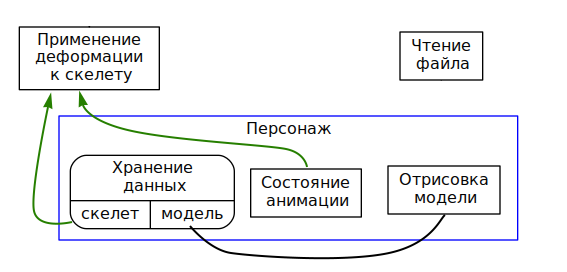
\includegraphics[width=0.8\textwidth]{block_diagram.png}
    \caption{\scriptsize{Схема логических блоков в программе}}
   %\label{fig:awesome_image}
\end{figure}    
    
\end{frame}



%=============================================================
\begin{frame}[fragile]
\frametitle{Описание системы, блок чтения файла}
	Заполнение структур данными из файла.
	    
    \smallskip
	С помощью библиотеки Assimp производим чтение из файла. Для оптимальной работы мы переводим данные в свои структуры. Другие функции этой библиотеки не используются.
	
\begin{scriptsize}
\begin{lstlisting}
public void LoadScene(byte[] filedata)
{
    using (MemoryStream fs = new MemoryStream(filedata))
    {
        _cur_scene = new SceneWrapper(ReadAssimpScene(fs, "dae"));
        _action = new Animator(_cur_scene.Animations[0]);
        BoneNode bones = _cur_scene.BuildBoneNodes("Armature");
        Node mesh = _cur_scene.FindNode("Mesh");
        ActionState state = new ActionState();
        _enttity = new Entity(_cur_scene, mesh, bones, state);
    }
}
\end{lstlisting}
\end{scriptsize}
		
\end{frame}



%=============================================================
\begin{frame}
\frametitle{Описание системы, блок состояния анимации}	
	Хранит состояние анимации. Наиболее важные поля:
\begin{itemize}        
    \item Название трэка анимации.
	\item Настоящий момент времени в секундах.
	\item Индексы всех ключевых кадров и время каждого ключевого кадра.
\end{itemize}

    Есть фyнкция SetTime(\dots) для перехода к определенному моменту времени. Она находит интервал между ключевыми кадрами, подсчитывает величину интерполяции.
\end{frame}




%=============================================================
\begin{frame}[fragile]
\frametitle{Описание системы, блок хранения данных}
\begin{multicols}{2}
    Работает со скелетом и моделью. Реализует функции поиска костей в скелете или подмоделей в модели.
    
    \smallskip
    Функция BuildBones строит скелет по данным из модели (скелет как отдельный класс не существует, он определяеться корневой костью). 
    
    \columnbreak
    
\begin{figure}
\begin{scriptsize}
\begin{verbatim}
class BoneNode
{
    public string Name;
    public Matrix4 GlobalTransform;
    public Matrix4 LocalTransform;
    
    public BoneNode Parent;
    public List<BoneNode> Children;
    public BoneNode(Node assimp_node) { ... }
}
\end{verbatim}
\end{scriptsize}
\caption{Kласс описывающий кость скелета}
\end{figure}

\end{multicols}
\end{frame}


%=============================================================
\begin{frame}
\frametitle{Описание системы, блок деформации скелета}
    Применяет данные, описывающие (в матрицах поворота) новую позицию для каждой кости к костям из скелета. То есть, деформирует скелет в соответствии с моментом времени в анимации.
    
    \medskip
    На вход блока подается класс ActionState, содержащий информацию о состоянии анимации и корневая кость скелета.
\end{frame}


%=============================================================
\begin{frame}
\frametitle{Описание системы, блоки отрисовки модели}
	Загружает данные о модели в OpenGL.
	
    \smallskip
	Запрашивает OpenGL об отводе буферов памяти под вершины, нормали, цвета вершин и массив индексов.
    
    \smallskip
    Применяет свойства материала, например: цвет, коэффициент рассеивания света, коэффициент свечения и т.д.
    
    \smallskip
    Позволяет запросить у OpenGL указатель на созданные буфера памяти для их модификации.
\end{frame}


%=============================================================
\begin{frame}
\frametitle{Описание системы, блок прерсонажа}
    Объединяет компоненты необходимые для анимации одного персонажа. Хранит ссылки на скелет (корневую кость), состояние анимации (ActionState), на саму модель и на класс отрисовки модели (MeshDraw)
    
    \medskip
    В частности блок персонажа применяет трансформации из скелета к вершинам модели (взвешивая действие каждой кости на вершину) и модифицирует данные в буфере данных OpenGL, что и создает эффект анимации.

\end{frame}




%=============================================================
\begin{frame}
\frametitle{Результаты работы}
    \begin{center}            
    \begin{large}
    Демонстрация
    \end{large}
    \end{center}
\end{frame}



%=============================================================
\begin{frame}
\frametitle{Апробация работы}
    \begin{center}            
    \begin{large}
    ???
    \end{large}
    \end{center}
\end{frame}




%=============================================================
\begin{frame}
\frametitle{Выводы по работе}
    Пути дальнейшей работы:
\begin{enumerate} 
	\item Загрузка нескольких моделей
	\item Наложение матрицы трансформации на отдельные модели
	\item Выбор из нескольких трэков анимации
	\item Нанесение текстур
	\item Анимация на GPU
\end{enumerate}

\begin{figure}[h!]
    \flushright
    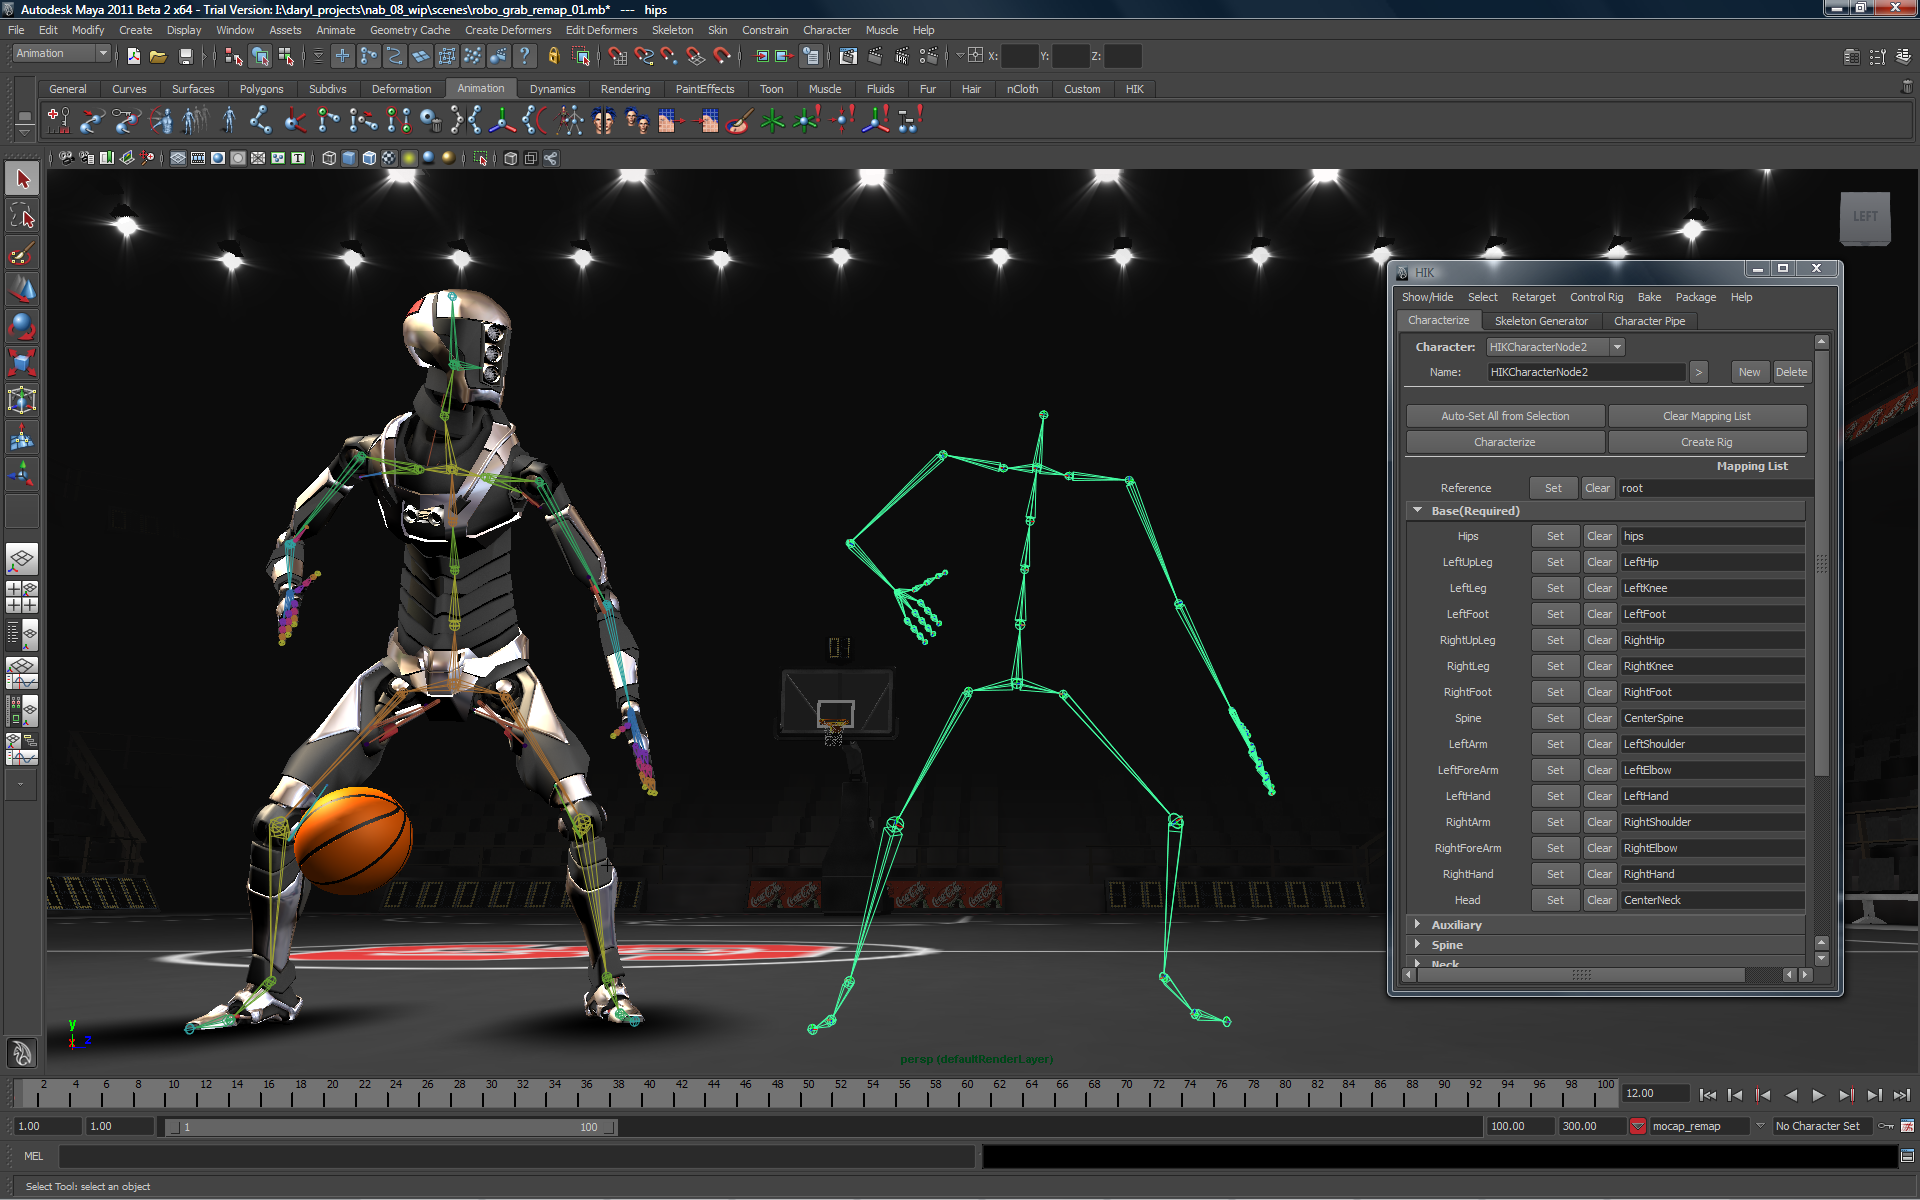
\includegraphics[width=0.6\textwidth]{win_maya.png}
    %\caption{\scriptsize{Схема логических блоков в программе}}
   %\label{fig:awesome_image}
\end{figure}

\end{frame}




%=============================================================
\begin{frame}
\frametitle{Список использованных источников}
\begin{itemize}
\item
Порев В.Н. Компьютерная графика. – СПб.: БХВ-Петербург, 2002. – 432 с.: ил.

\item 
Daniel S.D. Core Techniques and Algorithms in Game Programming/S.D. Daniel. - Springer, 2008 - 727 c.

\item
Документация OpenGL 3.3 [Электронный ресурс] // https://www.opengl.org/sdk/docs/man/ (Дата обращения: 21.10.2015, режим доступа: свободный)

\item
Рождерс Д. Алгоритмические основы машинной графики: Пер. с анг. - М.: Мир, 1989 - 512 с.
    
\end{itemize}
\end{frame}



\begin{frame}[c]
\begin{center}
\frametitle{\LARGE Спасибо за внимание!}

{\LARGE \inserttitle}

\bigskip

{\insertauthor}

\bigskip\bigskip

{\insertinstitute}

\bigskip\bigskip

{\large \insertdate}
\end{center}
\end{frame}

\end{document}
